% !TEX root =  main.tex

In questa sezione vengono descritte le componenti del sistema preso in
considerazione per la realizzazione del progetto Jolella. Tali descrizioni hanno
il solo scopo di informare, e non di porre vincoli sulle scelte implementative.
Alcuni di questi vincoli e limitazioni sono invece discussi nella
sezione~\ref{sec:implementation}, insieme alle motivazioni delle stesse.

\subsection{La rete Peer-To-Peer}
\label{subsec:p2p}

Il termine peer-to-peer~\cite{AS04,Balakrishnan:2003:LUD:606272.606299} si
riferisce ad una classe di sistemi ed applicazioni che utilizzano risorse
distribuite per eseguire una funzionalità (critica) in modo
decentralizzato~\cite{peer-to-peer}.

Ogni nodo in una rete P2P viene chiamato generalmente \textbf{peer}, ha la
medesima importanza e svolge le stesse funzioni di tutti gli altri nodi.

Le caratteristiche di un sistema P2P possono essere riassunte nelle seguenti:

\begin{itemize}

 \item i peer sono indipendenti (autonomi);

 \item ogni peer ha funzioni di \textbf{client} e di \textbf{server}
       contemporaneamente, e condivide delle risorse (in questo caso files);

 \item possono essere presenti dei nodi con funzionalità diverse rispetto agli
       altri, ad esempio per il monitoraggio o, in generale, per offrire operazioni
       specifiche;

 \item il sistema è \textbf{altamente distribuito}, il numero di peers può
       essere dell'ordine delle centinaia di migliaia;

 \item il sistema è \textbf{altamente dinamico}, un peer può entrare ed uscire
       dalla rete in ogni momento.

       \textbf{N.B.}

       \begin{itemize}

        \item le operazioni di ingresso/uscita (\textbf{join}/\textbf{leave}) dalla
              rete fanno parte dell'interfaccia di ogni peer.

       \end{itemize}

\end{itemize}

\subsubsection{Architetture di una rete P2P}

Esistono tre tipologie di reti distribuite peer-to-peer:

\begin{enumerate}

 \item Decentralizzate pure -- dove tutti i nodi sono peer, non esiste nessun
       coordinatore centralizzato. Ogni peer può funzionare come client e/o server.

 \item Parzialmente centralizzate -- in queste reti alcuni nodi (supernodi)
       facilitano l’interconnessione tra i peer, questi hanno, di solito, un indice
       locale centralizzato dei peer locali. Il
       pattern di comunicazione è: un peer comunica con il supernodo, che a sua volta
       comunica con gli altri peer.

 \item Decentralizzate ibride -- queste reti presentano un server centralizzato
       che facilita l’interazione tra i peer (servizio di \textbf{localizzazione}, ad
       esempio tramite \textbf{location}).

\end{enumerate}

\paragraph{Una rete P2P per la condivisione di files.} La condivisione di files
costituisce il principale utilizzo delle reti decentralizzate fin dagli anni
`90 (si parla di quasi il $30\%$ della rete Internet). Perchè una rete P2P sia
abilitata alla condivisione di files è necessario che ogni nodo esponga delle
funzionalità di \textbf{pubblicazione}, \textbf{ricerca} e \textbf{recupero}.

Vediamo un ``classico'' esempio di comunicazione tra due entità in una rete
peer-to-peer per la condivisione di un file:

\begin{enumerate}

 \item Alice esegue un \textbf{Client} P2P;

 \item Alice registra il suo contenuto nel sistema P2P;

 \item Alice cerca ``Hey Jude'';

 \item Il \textbf{Client} visualizza altri peer che hanno una copia di ``Hey
       Jude'';

 \item Alice sceglie uno, o più peer, per esempio Bob;

 \item il file viene copiato da Bob ad Alice;

 \item mentre Alice esegue il download, altri peer chiedono ad Alice l'upload
       di file.

\end{enumerate}

L'esempio riportato, senza pretesa di descrivere in modo completo il flusso di
comunicazioni, evidenzia alcune importanti proprietà che un \textbf{Client} di
una rete P2P per la condivisione files deve soddisfare. Esso, infatti, non solo
consente ad Alice di registrare un file per la sua condivisione ma, ``sotto il
tappeto'', si occupa, per esempio, di fare il \textit{join} della rete prima di
tutto il resto. Inoltre, permette ad Alice di copiare files condivisi da altri
utenti della rete e consente di individuare quali peer possiedono un determinato
file, tramite una ricerca basata su \textbf{keyword}.

Quest'ultimo problema, cioè quello della ricerca in una rete decentralizzata,
può essere ricondotto a quello del \textit{routing} o
instradamento~\footnote{Per una veloce lettura su questo argomento è possibile
 consultare la sezione dell'articolo relativo su Wikipedia:
 \url{https://it.wikipedia.org/wiki/Protocollo_di_routing}.}. Nei sistemi P2P per
la condivisione dei files il routing dipende dall'architettura del sistema
stesso, nel caso di sistemi decentralizzati ibridi, questo si effettua mediante
l'uso di una \textbf{directory centralizzata}~\footnote{Un esempio di programma
 di condivisione files basato su questa tecnica è il famoso Napster.}. Nel caso
invece di architetture decentralizzata pura, la ricerca utilizza il protocollo
di \textbf{flooding}.

\paragraph{Sistemi con directory centralizzata.} In questi sistemi un nodo
centralizzato, chiamato anche \textbf{directory server} possiede una mappa con
tutte le risorse dei peer, in un modo molto simile a quello che usano i sistemi
di ricerca dei computer che usiamo tutti i giorni (\textit{Siri},
\textit{Cortana}, etc.). Il servizio del (super-)nodo fornisce operazioni di
\textbf{discovery} dei peer e di \textbf{lookup} delle risorse.

Tra le criticità più importanti di questa tecnica esiste il costo di gestione
del server centralizzato, in termini di risorse, la scalabilità limitata, dovuta
all'approccio centralizzato (problemi di collo di bottiglia vengono spesso
riscrontrati in questi sitemi) e, di conseguenza, la presenza di un
\textit{single point of failure} nel sistema.

\begin{figure}[H]
 \centering
 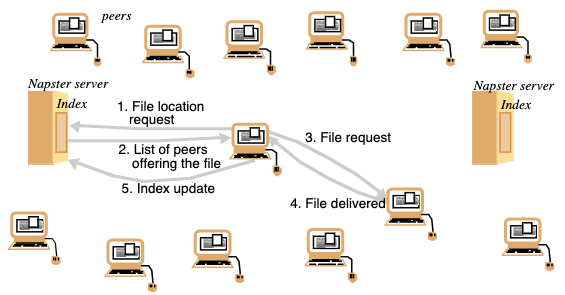
\includegraphics[width=0.8\textwidth]{directory}
 \caption{Rappresentazione grafica di un esempio di sistema con
  directory centralizzata. Fonte Uniroma.}
\end{figure}

\paragraph{Sistemi con ricerca flood-based.} Costituiscono l'approccio più
decentralizzato, in cui ogni peer propaga -- da qui il termine inglese
\textit{flood} -- la richiesta ai peer intorno a lui, che a loro volta inviano
la richiesta ai peer ``vicini'', escludendo  quello da cui hanno ricevuto la
richiesta. La risposta, una volta trovata, viene inviata direttamente al peer
originario della richiesta. I sistemi così configurati devono porre particolare
attenzione nella gestione della propagazione della richiesta, in quanto, senza
un'opportuna strategia di \textit{back-off}, essa potrebbe circolare
all'infinito. Una delle tecniche più usate è quella che utilizza un \textit{TTL}
(Time To Live), un intero contenuto in ogni query inviata. Ad ogni passaggio per
un nodo della rete, il peer decrementa questo TTL che, arrivato a 0, invalida la
richiesta e ferma la propagazione~\footnote{Anche in questo caso l'articolo di
Wikipedia mostra, brevemente, alcuni concetti chiave della tecnica di flooding e
del TTL, anche detto \textit{Hop
Count}~\url{https://en.wikipedia.org/wiki/Flooding_(computer_networking)}.}.

\begin{figure}[H]
 \centering
 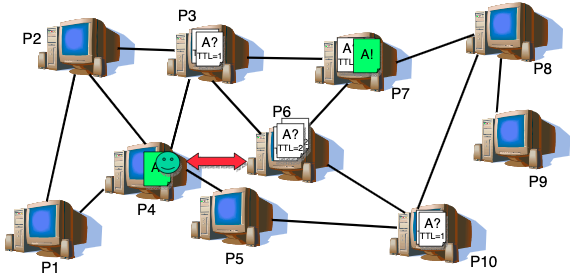
\includegraphics[width=0.85\textwidth]{flooding}
 \caption{Rappresentazione grafica di un esempio di sistema con
  directory centralizzata. Fonte Uniroma.}
\end{figure}

Note criticità del flooding riguardano la congestione della rete per il numero
di messaggi scambiati da sistemi in cui i messaggi di richiesta cercano di
esplorare l'intero insieme dei nodi. A questo è collegato anche il problema
della determinazione del raggio di ampiezza del flooding (e quindi il TTL). Non
esiste  quindi garanzia che venga interrogato il nodo che possiede la risorsa
pur sapendo che questa  esiste nella rete. Un'altra limitazione di questi
sistemi risiede nella nozione di ``vicinanza'' dei nodi, non è chiaro infatto
come definire questo  parametro, è spesso necessario effettuare dei  tentativi
per stabilire quale sia il valore migliore per un determinato sistema.
